% Options for packages loaded elsewhere
\PassOptionsToPackage{unicode}{hyperref}
\PassOptionsToPackage{hyphens}{url}
%
\documentclass[
]{article}
\usepackage{amsmath,amssymb}
\usepackage{iftex}
\ifPDFTeX
  \usepackage[T1]{fontenc}
  \usepackage[utf8]{inputenc}
  \usepackage{textcomp} % provide euro and other symbols
\else % if luatex or xetex
  \usepackage{unicode-math} % this also loads fontspec
  \defaultfontfeatures{Scale=MatchLowercase}
  \defaultfontfeatures[\rmfamily]{Ligatures=TeX,Scale=1}
\fi
\usepackage{lmodern}
\ifPDFTeX\else
  % xetex/luatex font selection
\fi
% Use upquote if available, for straight quotes in verbatim environments
\IfFileExists{upquote.sty}{\usepackage{upquote}}{}
\IfFileExists{microtype.sty}{% use microtype if available
  \usepackage[]{microtype}
  \UseMicrotypeSet[protrusion]{basicmath} % disable protrusion for tt fonts
}{}
\makeatletter
\@ifundefined{KOMAClassName}{% if non-KOMA class
  \IfFileExists{parskip.sty}{%
    \usepackage{parskip}
  }{% else
    \setlength{\parindent}{0pt}
    \setlength{\parskip}{6pt plus 2pt minus 1pt}}
}{% if KOMA class
  \KOMAoptions{parskip=half}}
\makeatother
\usepackage{xcolor}
\usepackage[margin=1in]{geometry}
\usepackage{color}
\usepackage{fancyvrb}
\newcommand{\VerbBar}{|}
\newcommand{\VERB}{\Verb[commandchars=\\\{\}]}
\DefineVerbatimEnvironment{Highlighting}{Verbatim}{commandchars=\\\{\}}
% Add ',fontsize=\small' for more characters per line
\usepackage{framed}
\definecolor{shadecolor}{RGB}{248,248,248}
\newenvironment{Shaded}{\begin{snugshade}}{\end{snugshade}}
\newcommand{\AlertTok}[1]{\textcolor[rgb]{0.94,0.16,0.16}{#1}}
\newcommand{\AnnotationTok}[1]{\textcolor[rgb]{0.56,0.35,0.01}{\textbf{\textit{#1}}}}
\newcommand{\AttributeTok}[1]{\textcolor[rgb]{0.13,0.29,0.53}{#1}}
\newcommand{\BaseNTok}[1]{\textcolor[rgb]{0.00,0.00,0.81}{#1}}
\newcommand{\BuiltInTok}[1]{#1}
\newcommand{\CharTok}[1]{\textcolor[rgb]{0.31,0.60,0.02}{#1}}
\newcommand{\CommentTok}[1]{\textcolor[rgb]{0.56,0.35,0.01}{\textit{#1}}}
\newcommand{\CommentVarTok}[1]{\textcolor[rgb]{0.56,0.35,0.01}{\textbf{\textit{#1}}}}
\newcommand{\ConstantTok}[1]{\textcolor[rgb]{0.56,0.35,0.01}{#1}}
\newcommand{\ControlFlowTok}[1]{\textcolor[rgb]{0.13,0.29,0.53}{\textbf{#1}}}
\newcommand{\DataTypeTok}[1]{\textcolor[rgb]{0.13,0.29,0.53}{#1}}
\newcommand{\DecValTok}[1]{\textcolor[rgb]{0.00,0.00,0.81}{#1}}
\newcommand{\DocumentationTok}[1]{\textcolor[rgb]{0.56,0.35,0.01}{\textbf{\textit{#1}}}}
\newcommand{\ErrorTok}[1]{\textcolor[rgb]{0.64,0.00,0.00}{\textbf{#1}}}
\newcommand{\ExtensionTok}[1]{#1}
\newcommand{\FloatTok}[1]{\textcolor[rgb]{0.00,0.00,0.81}{#1}}
\newcommand{\FunctionTok}[1]{\textcolor[rgb]{0.13,0.29,0.53}{\textbf{#1}}}
\newcommand{\ImportTok}[1]{#1}
\newcommand{\InformationTok}[1]{\textcolor[rgb]{0.56,0.35,0.01}{\textbf{\textit{#1}}}}
\newcommand{\KeywordTok}[1]{\textcolor[rgb]{0.13,0.29,0.53}{\textbf{#1}}}
\newcommand{\NormalTok}[1]{#1}
\newcommand{\OperatorTok}[1]{\textcolor[rgb]{0.81,0.36,0.00}{\textbf{#1}}}
\newcommand{\OtherTok}[1]{\textcolor[rgb]{0.56,0.35,0.01}{#1}}
\newcommand{\PreprocessorTok}[1]{\textcolor[rgb]{0.56,0.35,0.01}{\textit{#1}}}
\newcommand{\RegionMarkerTok}[1]{#1}
\newcommand{\SpecialCharTok}[1]{\textcolor[rgb]{0.81,0.36,0.00}{\textbf{#1}}}
\newcommand{\SpecialStringTok}[1]{\textcolor[rgb]{0.31,0.60,0.02}{#1}}
\newcommand{\StringTok}[1]{\textcolor[rgb]{0.31,0.60,0.02}{#1}}
\newcommand{\VariableTok}[1]{\textcolor[rgb]{0.00,0.00,0.00}{#1}}
\newcommand{\VerbatimStringTok}[1]{\textcolor[rgb]{0.31,0.60,0.02}{#1}}
\newcommand{\WarningTok}[1]{\textcolor[rgb]{0.56,0.35,0.01}{\textbf{\textit{#1}}}}
\usepackage{graphicx}
\makeatletter
\def\maxwidth{\ifdim\Gin@nat@width>\linewidth\linewidth\else\Gin@nat@width\fi}
\def\maxheight{\ifdim\Gin@nat@height>\textheight\textheight\else\Gin@nat@height\fi}
\makeatother
% Scale images if necessary, so that they will not overflow the page
% margins by default, and it is still possible to overwrite the defaults
% using explicit options in \includegraphics[width, height, ...]{}
\setkeys{Gin}{width=\maxwidth,height=\maxheight,keepaspectratio}
% Set default figure placement to htbp
\makeatletter
\def\fps@figure{htbp}
\makeatother
\setlength{\emergencystretch}{3em} % prevent overfull lines
\providecommand{\tightlist}{%
  \setlength{\itemsep}{0pt}\setlength{\parskip}{0pt}}
\setcounter{secnumdepth}{-\maxdimen} % remove section numbering
\ifLuaTeX
  \usepackage{selnolig}  % disable illegal ligatures
\fi
\IfFileExists{bookmark.sty}{\usepackage{bookmark}}{\usepackage{hyperref}}
\IfFileExists{xurl.sty}{\usepackage{xurl}}{} % add URL line breaks if available
\urlstyle{same}
\hypersetup{
  pdftitle={Exe2},
  hidelinks,
  pdfcreator={LaTeX via pandoc}}

\title{Exe2}
\author{}
\date{\vspace{-2.5em}2024-04-16}

\begin{document}
\maketitle

\emph{Exercise 1} - Discrete random variable

\begin{itemize}
\tightlist
\item
  The probability distribution function of a discrete variable \emph{k}
  is given by the \emph{zero-truncated} Poisson distribution: \[
  P(k) = \frac{\lambda^k e^{- \lambda}}{k! (1 - e^{-\lambda})}
  \]
\end{itemize}

\begin{enumerate}
\def\labelenumi{\arabic{enumi})}
\tightlist
\item
  Write the R functions for the probability density and cumulative
  distribution functions, using the R naming convention.
\end{enumerate}

\begin{itemize}
\tightlist
\item
  Assuming \(\lambda = 1.4\),
\end{itemize}

\begin{enumerate}
\def\labelenumi{\arabic{enumi})}
\setcounter{enumi}{1}
\tightlist
\item
  Produce two plots showing the pdf and cdf, separately.
\end{enumerate}

\begin{Shaded}
\begin{Highlighting}[]
\DocumentationTok{\#\# First let\textquotesingle{}s define the zero truncated poisson function}
\DocumentationTok{\#\# Remember that x is indeed a vector of n components }

\NormalTok{dpoisz }\OtherTok{\textless{}{-}} \ControlFlowTok{function}\NormalTok{(x, lambda) \{}
\NormalTok{    pmf }\OtherTok{\textless{}{-}}\NormalTok{ (lambda}\SpecialCharTok{\^{}}\NormalTok{x }\SpecialCharTok{*} \FunctionTok{exp}\NormalTok{(}\SpecialCharTok{{-}}\NormalTok{lambda) }\SpecialCharTok{/}\NormalTok{ (}\FunctionTok{factorial}\NormalTok{(x) }\SpecialCharTok{*}\NormalTok{ (}\DecValTok{1} \SpecialCharTok{{-}} \FunctionTok{exp}\NormalTok{(}\SpecialCharTok{{-}}\NormalTok{lambda))))}
  \FunctionTok{return}\NormalTok{(pmf)}
\NormalTok{\}}

\DocumentationTok{\#\# Let\textquotesingle{}s now define the cumulative distribution function}

\NormalTok{ppoisz }\OtherTok{\textless{}{-}} \ControlFlowTok{function}\NormalTok{(k, lambda) \{}
  
\NormalTok{  cdf }\OtherTok{\textless{}{-}} \FunctionTok{rep}\NormalTok{(}\DecValTok{0}\NormalTok{, }\FunctionTok{length}\NormalTok{(k))}
  
  \ControlFlowTok{for}\NormalTok{ (i }\ControlFlowTok{in} \DecValTok{1}\SpecialCharTok{:}\FunctionTok{length}\NormalTok{(k)) \{}
\NormalTok{    cdf[i] }\OtherTok{\textless{}{-}} \FunctionTok{sum}\NormalTok{(}\FunctionTok{dpoisz}\NormalTok{(}\DecValTok{1}\SpecialCharTok{:}\NormalTok{k[i], lambda))}
    
\NormalTok{  \}}
  \FunctionTok{return}\NormalTok{(cdf)}
\NormalTok{\}}


\NormalTok{N\_samples }\OtherTok{\textless{}{-}} \DecValTok{100}

\NormalTok{x }\OtherTok{\textless{}{-}} \DecValTok{1}\SpecialCharTok{:}\DecValTok{15}
\NormalTok{lambda }\OtherTok{\textless{}{-}} \FloatTok{1.4}


\FunctionTok{plot}\NormalTok{(}\FunctionTok{dpoisz}\NormalTok{(x, lambda), }\AttributeTok{type =} \StringTok{\textquotesingle{}s\textquotesingle{}}\NormalTok{, }\AttributeTok{lwd =} \DecValTok{2}\NormalTok{,}
     \AttributeTok{main =} \StringTok{\textquotesingle{}Poisson probability function (λ = 1.4)\textquotesingle{}}\NormalTok{,}
     \AttributeTok{ylab =} \StringTok{\textquotesingle{}P(X = x)\textquotesingle{}}\NormalTok{, }\AttributeTok{xlab =} \StringTok{\textquotesingle{}Number of events\textquotesingle{}}\NormalTok{,}
     \AttributeTok{ylim =} \FunctionTok{c}\NormalTok{(}\DecValTok{0}\NormalTok{, }\FloatTok{0.5}\NormalTok{), }
     \AttributeTok{xlim =} \FunctionTok{c}\NormalTok{(}\DecValTok{0}\NormalTok{, }\DecValTok{15}\NormalTok{)}
\NormalTok{     )}
\end{Highlighting}
\end{Shaded}

\begin{verbatim}
## Warning in title(...): conversione fallita da 'Poisson probability function (λ
## = 1.4)' in 'mbcsToSbcs': punto sostituito per <ce>
\end{verbatim}

\begin{verbatim}
## Warning in title(...): conversione fallita da 'Poisson probability function (λ
## = 1.4)' in 'mbcsToSbcs': punto sostituito per <bb>
\end{verbatim}

\begin{Shaded}
\begin{Highlighting}[]
\FunctionTok{lines}\NormalTok{(}\FunctionTok{dpoisz}\NormalTok{(x, lambda), }\AttributeTok{type =} \StringTok{\textquotesingle{}l\textquotesingle{}}\NormalTok{, }\AttributeTok{lty =} \DecValTok{2}\NormalTok{, }\AttributeTok{lwd =} \DecValTok{2}\NormalTok{, }\AttributeTok{col =} \StringTok{\textquotesingle{}red\textquotesingle{}}\NormalTok{)}
\FunctionTok{grid}\NormalTok{()}
\end{Highlighting}
\end{Shaded}

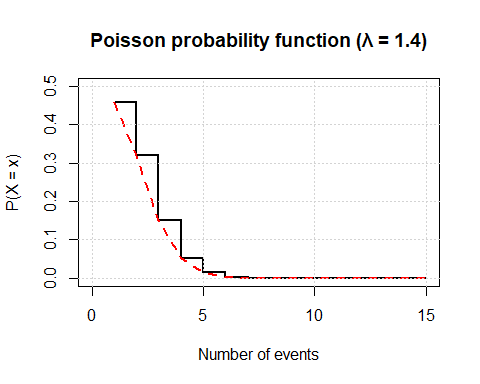
\includegraphics{Diorio_exe2_files/figure-latex/unnamed-chunk-1-1.pdf}

\begin{Shaded}
\begin{Highlighting}[]
\CommentTok{\#legend(\textquotesingle{}topright\textquotesingle{}, legend = \textquotesingle{}λ = 1.4\textquotesingle{}, col = \textquotesingle{}black\textquotesingle{}, lwd = 1, bty = \textquotesingle{}n\textquotesingle{})}
\end{Highlighting}
\end{Shaded}

\begin{Shaded}
\begin{Highlighting}[]
\CommentTok{\#{-}{-}{-}{-}{-}{-}{-}{-}{-}{-}{-}}
\CommentTok{\# lambda: 1.4}
\CommentTok{\#{-}{-}{-}{-}{-}{-}{-}{-}{-}{-}{-}}
\NormalTok{lambda }\OtherTok{\textless{}{-}} \FloatTok{1.4}
\NormalTok{k }\OtherTok{\textless{}{-}} \DecValTok{1}\SpecialCharTok{:}\DecValTok{15}


\FunctionTok{plot}\NormalTok{(}\FunctionTok{ppoisz}\NormalTok{(k, lambda), }\AttributeTok{type =} \StringTok{"s"}\NormalTok{, }\AttributeTok{lwd =} \DecValTok{2}\NormalTok{,}
     \AttributeTok{main =} \StringTok{"Cumulative distribution function (λ = 1.4)"}\NormalTok{,}
     \AttributeTok{xlab =} \StringTok{"Number of events"}\NormalTok{, }\AttributeTok{ylab =} \StringTok{"F(x)"}\NormalTok{, }\AttributeTok{col =} \DecValTok{2}\NormalTok{,}
     \AttributeTok{ylim =} \FunctionTok{c}\NormalTok{(}\FunctionTok{min}\NormalTok{(}\FunctionTok{ppoisz}\NormalTok{(k, lambda)), }\FunctionTok{max}\NormalTok{(}\FunctionTok{ppoisz}\NormalTok{(k, lambda)))}
\NormalTok{     )}
\end{Highlighting}
\end{Shaded}

\begin{verbatim}
## Warning in title(...): conversione fallita da 'Cumulative distribution function
## (λ = 1.4)' in 'mbcsToSbcs': punto sostituito per <ce>
\end{verbatim}

\begin{verbatim}
## Warning in title(...): conversione fallita da 'Cumulative distribution function
## (λ = 1.4)' in 'mbcsToSbcs': punto sostituito per <bb>
\end{verbatim}

\begin{Shaded}
\begin{Highlighting}[]
\FunctionTok{grid}\NormalTok{()}
\end{Highlighting}
\end{Shaded}

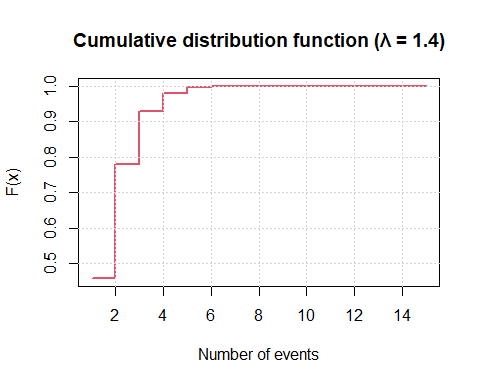
\includegraphics{Diorio_exe2_files/figure-latex/unnamed-chunk-2-1.pdf}

\begin{enumerate}
\def\labelenumi{\arabic{enumi})}
\setcounter{enumi}{2}
\tightlist
\item
  Compute the mean value and variance of the probability distribution
  using R.
\end{enumerate}

\begin{Shaded}
\begin{Highlighting}[]
\NormalTok{k }\OtherTok{\textless{}{-}} \DecValTok{0}\SpecialCharTok{:}\DecValTok{100}
\NormalTok{pdf }\OtherTok{\textless{}{-}} \FunctionTok{dpoisz}\NormalTok{(k, lambda)}
\NormalTok{pdf}\FloatTok{.2} \OtherTok{\textless{}{-}} \FunctionTok{dpoisz}\NormalTok{(k}\SpecialCharTok{\^{}}\DecValTok{2}\NormalTok{, lambda)}

\NormalTok{mean\_value }\OtherTok{\textless{}{-}} \FunctionTok{sum}\NormalTok{(k }\SpecialCharTok{*} \FunctionTok{dpoisz}\NormalTok{(k, lambda))}


\FunctionTok{print}\NormalTok{(}\FunctionTok{sprintf}\NormalTok{(}\StringTok{\textquotesingle{}Mean: \%.3f\textquotesingle{}}\NormalTok{, mean\_value))}
\end{Highlighting}
\end{Shaded}

\begin{verbatim}
## [1] "Mean: 1.858"
\end{verbatim}

\begin{Shaded}
\begin{Highlighting}[]
\NormalTok{std\_value }\OtherTok{\textless{}{-}} \FunctionTok{sum}\NormalTok{(k}\SpecialCharTok{\^{}}\DecValTok{2} \SpecialCharTok{*} \FunctionTok{dpoisz}\NormalTok{(k, lambda)) }\SpecialCharTok{{-}}\NormalTok{ mean\_value}\SpecialCharTok{\^{}}\DecValTok{2}


\FunctionTok{print}\NormalTok{(}\FunctionTok{sprintf}\NormalTok{(}\StringTok{\textquotesingle{}Variance: \%.3f\textquotesingle{}}\NormalTok{, std\_value))}
\end{Highlighting}
\end{Shaded}

\begin{verbatim}
## [1] "Variance: 1.007"
\end{verbatim}

\begin{enumerate}
\def\labelenumi{\arabic{enumi})}
\setcounter{enumi}{3}
\tightlist
\item
  Generating a sample of random numbers from the given distribution
\end{enumerate}

\begin{Shaded}
\begin{Highlighting}[]
\NormalTok{k }\OtherTok{\textless{}{-}} \DecValTok{1}\SpecialCharTok{:}\DecValTok{1000}
\NormalTok{samples }\OtherTok{\textless{}{-}} \FunctionTok{sample}\NormalTok{(k, }\AttributeTok{size =} \DecValTok{10000}\NormalTok{, }\AttributeTok{replace =} \ConstantTok{TRUE}\NormalTok{, }\AttributeTok{prob =} \FunctionTok{dpoisz}\NormalTok{(k, lambda))}


\FunctionTok{hist}\NormalTok{(samples,}
     \AttributeTok{breaks =} \FunctionTok{seq}\NormalTok{(}\FunctionTok{min}\NormalTok{(samples), }\FunctionTok{max}\NormalTok{(samples), }\AttributeTok{by =} \DecValTok{1}\NormalTok{),}
     \AttributeTok{main =} \StringTok{\textquotesingle{}Random samples from the zero truncated poisson distribution\textquotesingle{}}\NormalTok{, }
     \AttributeTok{xlab =} \StringTok{\textquotesingle{}Samples\textquotesingle{}}\NormalTok{, }\AttributeTok{ylab =} \StringTok{\textquotesingle{}Frequency\textquotesingle{}}\NormalTok{, }
     \AttributeTok{col =} \StringTok{\textquotesingle{}cyan\textquotesingle{}}\NormalTok{)}


\FunctionTok{abline}\NormalTok{(}\AttributeTok{v =}\NormalTok{ mean\_value, }\AttributeTok{col =} \StringTok{\textquotesingle{}red\textquotesingle{}}\NormalTok{, }\AttributeTok{lty =} \DecValTok{2}\NormalTok{, }\AttributeTok{lw =} \FloatTok{2.5}\NormalTok{)}
\CommentTok{\#lines(dpoisz(k, lambda), type = \textquotesingle{}l\textquotesingle{}, lty = 2, lwd = 2, col = \textquotesingle{}black\textquotesingle{})}
\FunctionTok{legend}\NormalTok{(}\StringTok{\textquotesingle{}topright\textquotesingle{}}\NormalTok{, }\AttributeTok{legend =} \FunctionTok{sprintf}\NormalTok{(}\StringTok{\textquotesingle{}Mean = \%.3f\textquotesingle{}}\NormalTok{, mean\_value), }\AttributeTok{col =} \StringTok{\textquotesingle{}red\textquotesingle{}}\NormalTok{, }\AttributeTok{lty =} \DecValTok{2}\NormalTok{, }\AttributeTok{lw =} \FloatTok{2.5}\NormalTok{)}
\FunctionTok{grid}\NormalTok{()}
\end{Highlighting}
\end{Shaded}

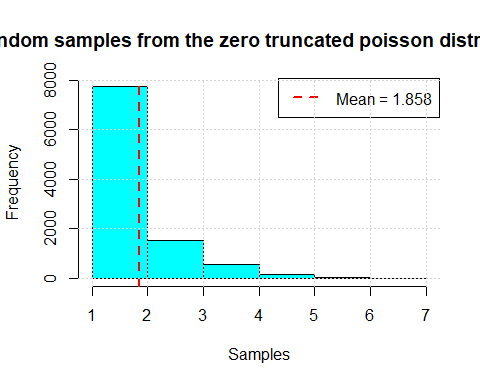
\includegraphics{Diorio_exe2_files/figure-latex/unnamed-chunk-4-1.pdf}

\emph{Exercise 2} - Continuous random variable

\begin{itemize}
\tightlist
\item
  The energy distribution of CR muons at sea level can be approximated
  as follows:
\end{itemize}

\[
\begin{cases}
p(E) = N \ \ &for \ \  E < E_0 \\
p(E ) = (E - E_0 + 1) ^ {- {\gamma}} \ \  &for  \ \ E\  \ge  \ E_0
\end{cases}
\]

where \(E_0 \ =\  7.25\  GeV\) and \(\gamma\  =\  2.7\).

\begin{enumerate}
\def\labelenumi{\alph{enumi})}
\item
  Compute the normalization factor N using R.
\item
  Plot the probability density function in R.
\item
  Plot the cumulative density function in R.
\item
  Compute the mean value using R.
\item
  {[} \(\textbf{Optional}\) {]} Generate \(10^6\) random numbers from
  this distribution, show them in an histogram and superimpose the pdf (
  with a line or with a sufficient number of points).
\end{enumerate}

\begin{Shaded}
\begin{Highlighting}[]
\DocumentationTok{\#\# R Markdown}
\CommentTok{\# To compute the normalization factor we need the integral }
\CommentTok{\# Let\textquotesingle{}s first define the probability distribution}

\NormalTok{p }\OtherTok{\textless{}{-}} \ControlFlowTok{function}\NormalTok{(E, N, E\_0, gamma) \{}
  \ControlFlowTok{if}\NormalTok{ (E }\SpecialCharTok{\textless{}}\NormalTok{ E\_0) \{}
    \FunctionTok{return}\NormalTok{(N)}
\NormalTok{  \} }\ControlFlowTok{else}\NormalTok{ \{}
    \FunctionTok{return}\NormalTok{(N }\SpecialCharTok{*}\NormalTok{ (E }\SpecialCharTok{{-}}\NormalTok{ E\_0 }\SpecialCharTok{+} \DecValTok{1}\NormalTok{) }\SpecialCharTok{\^{}}\NormalTok{ (}\SpecialCharTok{{-}}\NormalTok{gamma))}
\NormalTok{  \}}
\NormalTok{\}}

\NormalTok{E\_0 }\OtherTok{\textless{}{-}} \FloatTok{7.25}
\NormalTok{gamma }\OtherTok{\textless{}{-}} \FloatTok{2.7}

\NormalTok{n\_steps }\OtherTok{\textless{}{-}} \DecValTok{100}
\NormalTok{dE }\OtherTok{\textless{}{-}}\NormalTok{ E\_0 }\SpecialCharTok{/}\NormalTok{ n\_steps}

\DocumentationTok{\#\# First we need to compute the integral of the distribution}
\NormalTok{summ }\OtherTok{\textless{}{-}} \DecValTok{0}
\ControlFlowTok{for}\NormalTok{ (i }\ControlFlowTok{in}\NormalTok{ n\_steps) \{}
\NormalTok{  summ }\OtherTok{\textless{}{-}}\NormalTok{ summ }\SpecialCharTok{+} \FunctionTok{p}\NormalTok{(dE, }\AttributeTok{N =} \DecValTok{1}\NormalTok{, E\_0, gamma)}
\NormalTok{\}}

\NormalTok{N }\OtherTok{\textless{}{-}}\NormalTok{ summ }\SpecialCharTok{/}\NormalTok{ E\_0}

\FunctionTok{print}\NormalTok{(}\FunctionTok{sprintf}\NormalTok{(}\StringTok{\textquotesingle{}Normalization factor: \%.3f \textquotesingle{}}\NormalTok{, N))}
\end{Highlighting}
\end{Shaded}

\begin{verbatim}
## [1] "Normalization factor: 0.138 "
\end{verbatim}

\begin{Shaded}
\begin{Highlighting}[]
\DocumentationTok{\#\# Let\textquotesingle{}s plot the probability density function in R}
\NormalTok{N\_steps }\OtherTok{\textless{}{-}} \DecValTok{100}

\NormalTok{E }\OtherTok{\textless{}{-}} \DecValTok{0}
\NormalTok{dE }\OtherTok{\textless{}{-}}\NormalTok{ E\_0 }\SpecialCharTok{/}\NormalTok{ N\_steps }
\NormalTok{E\_stored }\OtherTok{\textless{}{-}} \FunctionTok{numeric}\NormalTok{(N\_steps }\SpecialCharTok{*} \DecValTok{2}\NormalTok{)}
\NormalTok{pdf }\OtherTok{\textless{}{-}} \FunctionTok{numeric}\NormalTok{(N\_steps }\SpecialCharTok{*} \DecValTok{2}\NormalTok{)}

\ControlFlowTok{for}\NormalTok{ (i }\ControlFlowTok{in} \DecValTok{1}\SpecialCharTok{:}\NormalTok{(N\_steps }\SpecialCharTok{*} \DecValTok{2}\NormalTok{)) \{}
\NormalTok{  E\_stored[i] }\OtherTok{\textless{}{-}}\NormalTok{ E}
\NormalTok{  pdf[i] }\OtherTok{\textless{}{-}}  \FunctionTok{p}\NormalTok{(E, N, E\_0, gamma)}
\NormalTok{  E }\OtherTok{\textless{}{-}}\NormalTok{ E }\SpecialCharTok{+}\NormalTok{ dE}
\NormalTok{\}}

\FunctionTok{plot}\NormalTok{(E\_stored, pdf, }
     \AttributeTok{xlab =} \StringTok{\textquotesingle{}Energy [GeV]\textquotesingle{}}\NormalTok{,}
     \AttributeTok{ylab =} \StringTok{\textquotesingle{}p(E)\textquotesingle{}}\NormalTok{, }
     \AttributeTok{type  =}\StringTok{\textquotesingle{}l\textquotesingle{}}\NormalTok{, }\AttributeTok{lwd =} \DecValTok{2}\NormalTok{, }
     \AttributeTok{main =} \StringTok{\textquotesingle{}Probability Density Function\textquotesingle{}}\NormalTok{)}
\FunctionTok{grid}\NormalTok{()}
\end{Highlighting}
\end{Shaded}

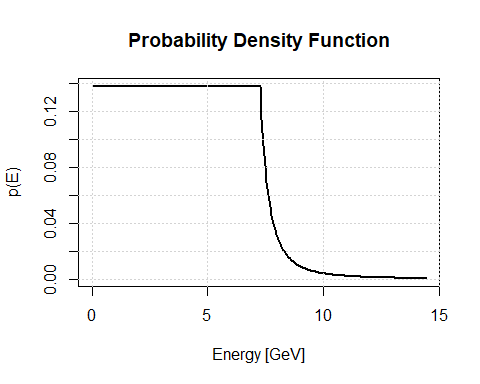
\includegraphics{Diorio_exe2_files/figure-latex/unnamed-chunk-6-1.pdf}

\begin{Shaded}
\begin{Highlighting}[]
\NormalTok{CDF }\OtherTok{\textless{}{-}} \FunctionTok{numeric}\NormalTok{(N\_steps }\SpecialCharTok{*} \DecValTok{2}\NormalTok{)}

\ControlFlowTok{for}\NormalTok{ (i }\ControlFlowTok{in}\NormalTok{ (}\DecValTok{1}\SpecialCharTok{:}\NormalTok{N\_steps }\SpecialCharTok{*} \DecValTok{2}\NormalTok{)) \{}
\NormalTok{  CDF[i] }\OtherTok{\textless{}{-}} \FunctionTok{sum}\NormalTok{(pdf[}\DecValTok{0}\SpecialCharTok{:}\NormalTok{i])}
\NormalTok{\}}

\FunctionTok{plot}\NormalTok{(E\_stored, CDF, }\AttributeTok{type =} \StringTok{\textquotesingle{}s\textquotesingle{}}\NormalTok{, }
     \AttributeTok{xlab =} \StringTok{\textquotesingle{}Energy [GeV]\textquotesingle{}}\NormalTok{, }\AttributeTok{ylab =} \StringTok{\textquotesingle{}CDF\textquotesingle{}}\NormalTok{, }
     \AttributeTok{main =} \StringTok{\textquotesingle{}Cumulative distribution function\textquotesingle{}}\NormalTok{,}
     \AttributeTok{col =} \StringTok{\textquotesingle{}black\textquotesingle{}}\NormalTok{, }\AttributeTok{lwd =} \DecValTok{2}\NormalTok{)}
\FunctionTok{grid}\NormalTok{()}
\end{Highlighting}
\end{Shaded}

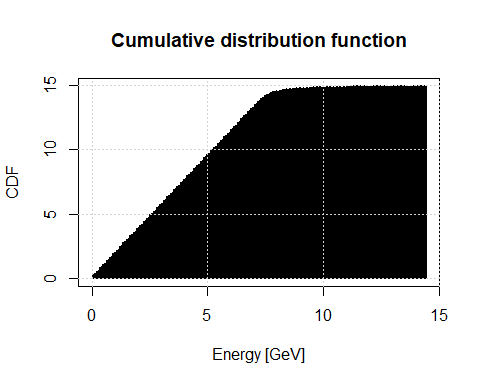
\includegraphics{Diorio_exe2_files/figure-latex/unnamed-chunk-7-1.pdf}

\begin{Shaded}
\begin{Highlighting}[]
\DocumentationTok{\#\# Compute the mean }

\NormalTok{E.x}\FloatTok{.1} \OtherTok{\textless{}{-}} \FunctionTok{integrate}\NormalTok{(}\ControlFlowTok{function}\NormalTok{(E) \{N }\SpecialCharTok{*}\NormalTok{ E\}, }\AttributeTok{lower =} \DecValTok{0}\NormalTok{, }\AttributeTok{upper =}\NormalTok{ E\_0)}\SpecialCharTok{$}\NormalTok{value}

\NormalTok{E.x}\FloatTok{.2} \OtherTok{\textless{}{-}} \FunctionTok{integrate}\NormalTok{(}\ControlFlowTok{function}\NormalTok{(E) \{N }\SpecialCharTok{*}\NormalTok{ E }\SpecialCharTok{*}\NormalTok{ (E }\SpecialCharTok{{-}}\NormalTok{ E\_0 }\SpecialCharTok{+} \DecValTok{1}\NormalTok{)}\SpecialCharTok{\^{}}\NormalTok{(}\SpecialCharTok{{-}}\NormalTok{gamma)\}, }\AttributeTok{lower =}\NormalTok{ E\_0, }\AttributeTok{upper =} \ConstantTok{Inf}\NormalTok{)}\SpecialCharTok{$}\NormalTok{value}

\NormalTok{integral }\OtherTok{\textless{}{-}}\NormalTok{ E.x}\FloatTok{.1} \SpecialCharTok{+}\NormalTok{ E.x}\FloatTok{.2}
\FunctionTok{print}\NormalTok{(}\FunctionTok{paste}\NormalTok{(}\FunctionTok{sprintf}\NormalTok{(}\StringTok{\textquotesingle{}Mean of the distribution: \%.3f\textquotesingle{}}\NormalTok{, E.x}\FloatTok{.1} \SpecialCharTok{+}\NormalTok{ E.x}\FloatTok{.2}\NormalTok{), }\StringTok{\textquotesingle{}GeV\textquotesingle{}}\NormalTok{))}
\end{Highlighting}
\end{Shaded}

\begin{verbatim}
## [1] "Mean of the distribution: 4.329 GeV"
\end{verbatim}

\emph{Exercise 3} - Suppose that the average number of accidents at an
intersection is two per day.

\begin{enumerate}
\def\labelenumi{\alph{enumi})}
\tightlist
\item
  Using Markov's inequality, find a bound for the probability that at
  least five accidents will occur tomorrow.
\end{enumerate}

From Markov's inequality we know that

\[
P(X \ge k) \le \frac{\mu}{k} 
\]

Applying in our case:

\[
P(X \ge 5) \le \frac{2}{5}
\]

b. Using Poisson random variables, calculate the probability that at
least five accidents will occur tomorrow. Compare this value with the
bound obtained in the previous point a).

Using a Poisson random variable we define:

\[
P(X \ge 5) = 1 - P(X \le 4)
\]

c. Let the variance of the number of accidents be two per day. Using
Chebyshev's inequality, find a bound on the probability that tomorrow at
least five accidents will occur.

Now applying the Chebyshev's inequality:

\[
P(|X \ - \ \mu| \ \ge k) \le \frac{\sigma^2}{k^2}
\]

where, in our case:

\[
\begin{cases}
Var(X) &= &2 \\ 
\mu &= &2
\end{cases}
\]

then:

\[
P(X \ - \ 2 \ge k) \ \le \ P(X - 2 \ge k) \ + \ P(-X \ + \ 2 \le  -  \ k) \ = \ P(|X - 2| \ge \ k) 
\]

so we apply the Chebishev's inequality with k = 3:

\[
P(|X \ - \ 2| \ \ge \ 3) \le \frac{2}{9}
\]

\begin{Shaded}
\begin{Highlighting}[]
\DocumentationTok{\#\# First let\textquotesingle{}s use Markov\textquotesingle{}s inequality }

\NormalTok{avg\_acc }\OtherTok{\textless{}{-}} \DecValTok{2}
\NormalTok{prob }\OtherTok{\textless{}{-}}\NormalTok{ avg\_acc }\SpecialCharTok{/} \DecValTok{5}

\FunctionTok{print}\NormalTok{(}\FunctionTok{paste}\NormalTok{(}\StringTok{\textquotesingle{}The probability of having at least 5 accidents is\textquotesingle{}}\NormalTok{, prob }\SpecialCharTok{*} \DecValTok{100}\NormalTok{, }\StringTok{\textquotesingle{}\%\textquotesingle{}}\NormalTok{))}
\end{Highlighting}
\end{Shaded}

\begin{verbatim}
## [1] "The probability of having at least 5 accidents is 40 %"
\end{verbatim}

\begin{Shaded}
\begin{Highlighting}[]
\DocumentationTok{\#\# Now let\textquotesingle{}s assume that each accident is described by a Poisson variable with lambda = 2}

\NormalTok{lambda }\OtherTok{\textless{}{-}} \DecValTok{2}

\DocumentationTok{\#\# P(N(t) = n) = (lambda * t)\^{}n * e\^{}({-}5t) / n! with t = 24/24 (tomorrow) = 1}
\DocumentationTok{\#\# P(N(1) \textgreater{}= 5) = 1 {-} P(N(1) = 0) {-} P(N(1) = 1) {-} P(N(1) = 2) {-} P(N(1) = 3) {-} ...}

\NormalTok{poisson\_prob }\OtherTok{\textless{}{-}} \FunctionTok{ppois}\NormalTok{(}\DecValTok{4}\NormalTok{, lambda)}
\FunctionTok{print}\NormalTok{(}\FunctionTok{paste}\NormalTok{(}\FunctionTok{sprintf}\NormalTok{(}\StringTok{\textquotesingle{}The probability given by the Poisson distribution is: \%.2f \textquotesingle{}}\NormalTok{, (}\DecValTok{1} \SpecialCharTok{{-}}\NormalTok{ poisson\_prob)}\SpecialCharTok{*} \DecValTok{100}\NormalTok{), }\StringTok{\textquotesingle{}\%\textquotesingle{}}\NormalTok{))}
\end{Highlighting}
\end{Shaded}

\begin{verbatim}
## [1] "The probability given by the Poisson distribution is: 5.27  %"
\end{verbatim}

\begin{Shaded}
\begin{Highlighting}[]
\DocumentationTok{\#\# Now let\textquotesingle{}s use the Chebishev\textquotesingle{}s inequality }

\NormalTok{var\_x }\OtherTok{\textless{}{-}} \DecValTok{2} \CommentTok{\# {-}\textgreater{} sigma = 1}
\NormalTok{mu\_x }\OtherTok{\textless{}{-}} \DecValTok{2}

\DocumentationTok{\#\# P(|x {-} mu| \textgreater{}= r sigma) \textless{}= var/r\^{}2 sigma\^{}2 = 1/r\^{}2}
\DocumentationTok{\#\# Nel nostro caso sigma = 1, |x {-} mu| \textgreater{}= 3 sigma }

\NormalTok{cheb\_prob }\OtherTok{\textless{}{-}} \DecValTok{2} \SpecialCharTok{/} \DecValTok{9}

\FunctionTok{print}\NormalTok{(}\FunctionTok{paste}\NormalTok{(}\FunctionTok{sprintf}\NormalTok{(}\StringTok{\textquotesingle{}The Chebishev}\SpecialCharTok{\textbackslash{}\textquotesingle{}}\StringTok{s upper bound is of: \%.2f\textquotesingle{}}\NormalTok{, cheb\_prob }\SpecialCharTok{*} \DecValTok{100}\NormalTok{), }\StringTok{\textquotesingle{}\%\textquotesingle{}}\NormalTok{))}
\end{Highlighting}
\end{Shaded}

\begin{verbatim}
## [1] "The Chebishev's upper bound is of: 22.22 %"
\end{verbatim}

\emph{Exercise 4} - The waiting period from the time a book is ordered
until it is received is a random variable with mean seven days and
standard deviation two days. If Helen wants to be 95\% sure that she
receives a book by a certain date, how early should she order the book?

As before we can apply Chebyshev's inequality:

\[
P(|X \ - \mu| \ge \ r\sigma) \le \frac{1}{r^2} \  \\ 
P(|X \ - \mu| \le \ r \sigma) = 1 - P(|X \ - \mu| \ \ge \ r\sigma) \le  \ 1 - \frac{1}{r^2} = 0.95 \\    
\rightarrow \frac{1}{r^2} \ = 1 - 0.95 = 0.05 \rightarrow \ r = \sqrt(\frac{10^2}{5}) 
\]

\begin{Shaded}
\begin{Highlighting}[]
\NormalTok{mu\_x }\OtherTok{\textless{}{-}} \DecValTok{7} \CommentTok{\#days }
\NormalTok{sigma\_x }\OtherTok{\textless{}{-}} \DecValTok{2} 

\DocumentationTok{\#\# P(|x {-} mu\_x| \textless{}{-} sigma\_x ) = 0.95}
\DocumentationTok{\#\# P(|x {-} mu\_x| \textless{} r sigma) \textgreater{}= 1 {-} 1/r\^{}2 = 0.95 {-}\textgreater{} r = sqrt(10\^{}2 /5)}
\DocumentationTok{\#\# |x {-} 7| \textless{} r sigma {-}\textgreater{} x \textgreater{} 7 {-} r sigma}

\NormalTok{r }\OtherTok{\textless{}{-}} \FunctionTok{sqrt}\NormalTok{(}\DecValTok{10}\SpecialCharTok{\^{}}\DecValTok{2} \SpecialCharTok{/} \DecValTok{5}\NormalTok{) }\CommentTok{\# Z score = z * sigma (?? not sure)}
\NormalTok{x }\OtherTok{\textless{}{-}}\NormalTok{ mu\_x }\SpecialCharTok{+}\NormalTok{ r }\SpecialCharTok{*}\NormalTok{ sigma\_x}

\FunctionTok{print}\NormalTok{(}\FunctionTok{paste}\NormalTok{(}\FunctionTok{sprintf}\NormalTok{(}\StringTok{\textquotesingle{}She should order it at least: \%.0f\textquotesingle{}}\NormalTok{, x), }\StringTok{\textquotesingle{}days before\textquotesingle{}}\NormalTok{))}
\end{Highlighting}
\end{Shaded}

\begin{verbatim}
## [1] "She should order it at least: 16 days before"
\end{verbatim}

\emph{Exercise 5} - An ordinary deck of 52 cards is divided randomly
into 26 pairs. Using Chebyshev's inequality, find an upper bound for the
probability that, at most, 10 pairs consist of a black and a red card.

\begin{Shaded}
\begin{Highlighting}[]
\CommentTok{\# 10 coppie devono essere formate da una carta nera ed una rossa}
\CommentTok{\# 26 coppie possibili: 10 / 26 devono essere accoppiate }
\CommentTok{\# P(|x {-} mu\_x| \textgreater{}= r*sigma) \textless{}= 1 / r\^{}2 }
\CommentTok{\# mu\_x = 13}
\CommentTok{\# sigma\^{}2 = np(1{-}p) = 26 * (26/52 * 26/51) * (1 {-} 26/52 * 26/51)}
\CommentTok{\# k = |10 {-}mu| / sigma =  3 / sigma\^{}2 }
\DocumentationTok{\#\# Let\textquotesingle{}s simulate the deck }

\NormalTok{Generating\_deck }\OtherTok{\textless{}{-}} \ControlFlowTok{function}\NormalTok{() \{}
\NormalTok{  N }\OtherTok{\textless{}{-}} \DecValTok{52}
\NormalTok{  mazzo }\OtherTok{\textless{}{-}} \FunctionTok{c}\NormalTok{(}\FunctionTok{rep}\NormalTok{(}\DecValTok{0}\NormalTok{, N}\SpecialCharTok{/}\DecValTok{2}\NormalTok{), }\FunctionTok{rep}\NormalTok{(}\DecValTok{1}\NormalTok{, N}\SpecialCharTok{/}\DecValTok{2}\NormalTok{))}
\NormalTok{  mazzo }\OtherTok{\textless{}{-}}\NormalTok{ mazzo[}\FunctionTok{sample}\NormalTok{(}\FunctionTok{length}\NormalTok{(mazzo))]}
\NormalTok{  y }\OtherTok{\textless{}{-}} \DecValTok{0}
  \ControlFlowTok{for}\NormalTok{ (i }\ControlFlowTok{in} \DecValTok{1}\SpecialCharTok{:}\NormalTok{(N}\SpecialCharTok{/}\DecValTok{2}\NormalTok{))\{}
    \ControlFlowTok{if}\NormalTok{ (mazzo[i] }\SpecialCharTok{+}\NormalTok{ mazzo[i}\SpecialCharTok{+}\NormalTok{N}\SpecialCharTok{/}\DecValTok{2}\NormalTok{] }\SpecialCharTok{==} \DecValTok{1}\NormalTok{)\{}
\NormalTok{      y }\OtherTok{\textless{}{-}}\NormalTok{ y }\SpecialCharTok{+} \DecValTok{1}
\NormalTok{    \}}
\NormalTok{  \}}
  \FunctionTok{return}\NormalTok{(y)}
\NormalTok{\}}

\NormalTok{N\_campioni }\OtherTok{\textless{}{-}} \DecValTok{100000}
\NormalTok{campioni }\OtherTok{\textless{}{-}} \FunctionTok{rep}\NormalTok{(}\DecValTok{0}\NormalTok{, N\_campioni)}
\ControlFlowTok{for}\NormalTok{ (i }\ControlFlowTok{in} \DecValTok{1}\SpecialCharTok{:}\NormalTok{N\_campioni) \{}
\NormalTok{  campioni[i] }\OtherTok{\textless{}{-}} \FunctionTok{Generating\_deck}\NormalTok{()}
\NormalTok{\}}

\FunctionTok{hist}\NormalTok{(campioni, }\AttributeTok{breaks =} \FunctionTok{seq}\NormalTok{(}\FunctionTok{min}\NormalTok{(campioni) }\SpecialCharTok{{-}} \FloatTok{0.5}\NormalTok{, }
                            \FunctionTok{max}\NormalTok{(campioni) }\SpecialCharTok{+} \FloatTok{0.5}\NormalTok{, }\AttributeTok{by =} \DecValTok{1}\NormalTok{), }\AttributeTok{main =} \StringTok{\textquotesingle{}Samples distribution\textquotesingle{}}\NormalTok{, }\AttributeTok{xlab =} \StringTok{\textquotesingle{}Samples\textquotesingle{}}\NormalTok{, }\AttributeTok{ylab =} \StringTok{\textquotesingle{}Frequency\textquotesingle{}}\NormalTok{)}

\NormalTok{media }\OtherTok{\textless{}{-}} \FunctionTok{mean}\NormalTok{(campioni)}
\NormalTok{deviazione\_standard }\OtherTok{\textless{}{-}} \FunctionTok{sd}\NormalTok{(campioni)}
\NormalTok{delta }\OtherTok{\textless{}{-}} \DecValTok{10} \SpecialCharTok{{-}}\NormalTok{ media }
\NormalTok{k }\OtherTok{\textless{}{-}}\NormalTok{ delta }\SpecialCharTok{/}\NormalTok{ deviazione\_standard}
\NormalTok{limite\_superiore }\OtherTok{\textless{}{-}} \DecValTok{1} \SpecialCharTok{/}\NormalTok{ k}\SpecialCharTok{\^{}}\DecValTok{2} 

\FunctionTok{abline}\NormalTok{(}\AttributeTok{v =}\NormalTok{ media, }\AttributeTok{col =} \StringTok{\textquotesingle{}red\textquotesingle{}}\NormalTok{, }\AttributeTok{lty =} \DecValTok{2}\NormalTok{, }\AttributeTok{lw =} \FloatTok{2.5}\NormalTok{)}
\FunctionTok{abline}\NormalTok{(}\AttributeTok{v =} \FunctionTok{c}\NormalTok{(media }\SpecialCharTok{{-}}\NormalTok{ deviazione\_standard, media }\SpecialCharTok{+}\NormalTok{ deviazione\_standard), }\AttributeTok{col =} \StringTok{"black"}\NormalTok{, }\AttributeTok{lty =} \DecValTok{2}\NormalTok{, }\AttributeTok{lw =} \DecValTok{1}\NormalTok{)}
\FunctionTok{print}\NormalTok{(}\FunctionTok{paste}\NormalTok{(}\FunctionTok{sprintf}\NormalTok{(}\StringTok{\textquotesingle{}The upper bound given by Chebyshev is of: \%.2f\textquotesingle{}}\NormalTok{, limite\_superiore }\SpecialCharTok{*} \DecValTok{100}\NormalTok{), }\StringTok{\textquotesingle{}\%\textquotesingle{}}\NormalTok{))}
\end{Highlighting}
\end{Shaded}

\begin{verbatim}
## [1] "The upper bound given by Chebyshev is of: 62.67 %"
\end{verbatim}

\begin{Shaded}
\begin{Highlighting}[]
\FunctionTok{legend}\NormalTok{(}\StringTok{\textquotesingle{}topright\textquotesingle{}}\NormalTok{, }\AttributeTok{legend =} \FunctionTok{c}\NormalTok{(}\StringTok{\textquotesingle{}Media\textquotesingle{}}\NormalTok{, }\StringTok{\textquotesingle{}Deviazione standard\textquotesingle{}}\NormalTok{),}
       \AttributeTok{col =} \FunctionTok{c}\NormalTok{(}\StringTok{\textquotesingle{}red\textquotesingle{}}\NormalTok{, }\StringTok{\textquotesingle{}black\textquotesingle{}}\NormalTok{), }\AttributeTok{lty =} \DecValTok{2}\NormalTok{, }\AttributeTok{cex =} \FloatTok{0.8}\NormalTok{)}
\end{Highlighting}
\end{Shaded}

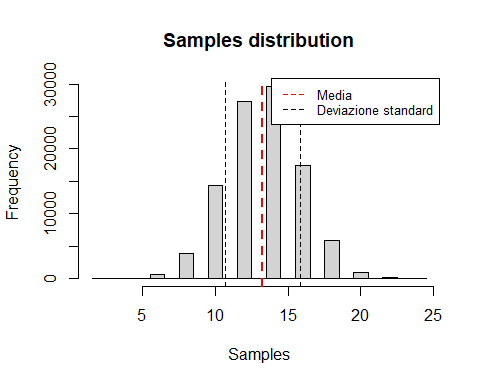
\includegraphics{Diorio_exe2_files/figure-latex/unnamed-chunk-11-1.pdf}

\emph{Exercise 6} - In a stationary bus at the departure station, a
passenger gets on the bus, on average, every 30 seconds.

\begin{enumerate}
\def\labelenumi{\alph{enumi})}
\tightlist
\item
  Compute the probability of getting more than 6 passengers after 2
  minutes. Evaluate the probability of having less than 4 passengers
  after 3 minutes.
\end{enumerate}

The probability is given by a Poisson distribution with
\(\lambda = \frac{1}{30}\). The probability of having more than 6
passengers will be given by:

\[
P(X \ge 5) = 1 - P(X \le 6) = 1 \ - \ Pois(\lambda = 40)
\]

while the probability of having less than 4 passengers is:

\[
P(X \le 4) \ = \ Pois(\lambda = 60)
\]

b. Simulate the distribution of the arrival time of the third passenger
and superimpose the corresponding pdf.

The arrival time of the passengers can be represented with an
exponential distribution where:

\[
\Delta t_i = Exp(\lambda) \ \rightarrow \ T_3 = \sum_{i=1}^3 \Delta t_i 
\]

where \(T_3\) is the arrival time of the third passenger. The sum of the
components will be distributed as the Erlang distribution.

c. Repeat the procedure of point b) for the difference in arrival time
between the fifth and the first passenger.

Now we evaluate the time difference, also distributed as an Erlang
distribution:

\[
\Delta T = T_5 \ - \ T_1 = \sum_{i=1}^5\Delta t_i \ - \ \Delta t_1 = \sum_{i=1}^4 \Delta t_i
\]

\begin{Shaded}
\begin{Highlighting}[]
\DocumentationTok{\#\# Consideriamo eventi scorrelati, ogni evento è indipendente dagli altri }

\NormalTok{lambda }\OtherTok{\textless{}{-}} \DecValTok{1}\SpecialCharTok{/}\FloatTok{30.}

\NormalTok{prob1 }\OtherTok{\textless{}{-}} \DecValTok{1} \SpecialCharTok{{-}} \FunctionTok{ppois}\NormalTok{(}\DecValTok{6}\NormalTok{, lambda }\SpecialCharTok{*} \DecValTok{120}\NormalTok{) }\CommentTok{\#seconds}
\NormalTok{prob2 }\OtherTok{\textless{}{-}} \FunctionTok{ppois}\NormalTok{(}\DecValTok{4}\NormalTok{, lambda }\SpecialCharTok{*} \DecValTok{180}\NormalTok{)}

\FunctionTok{print}\NormalTok{(}\FunctionTok{paste}\NormalTok{(}\FunctionTok{sprintf}\NormalTok{(}\StringTok{\textquotesingle{}The probability of getting more than 6 passengers after 2 minutes is of: \%.2f\textquotesingle{}}\NormalTok{, prob1 }\SpecialCharTok{*} \DecValTok{100}\NormalTok{), }\StringTok{\textquotesingle{}\%\textquotesingle{}}\NormalTok{))}
\end{Highlighting}
\end{Shaded}

\begin{verbatim}
## [1] "The probability of getting more than 6 passengers after 2 minutes is of: 11.07 %"
\end{verbatim}

\begin{Shaded}
\begin{Highlighting}[]
\FunctionTok{print}\NormalTok{(}\FunctionTok{paste}\NormalTok{(}\FunctionTok{sprintf}\NormalTok{(}\StringTok{\textquotesingle{}The probability of having less than 4 passengers after 3 minutes is given by: \%.2f\textquotesingle{}}\NormalTok{, prob2 }\SpecialCharTok{*} \DecValTok{100}\NormalTok{), }\StringTok{\textquotesingle{}\%\textquotesingle{}}\NormalTok{))}
\end{Highlighting}
\end{Shaded}

\begin{verbatim}
## [1] "The probability of having less than 4 passengers after 3 minutes is given by: 28.51 %"
\end{verbatim}

\begin{Shaded}
\begin{Highlighting}[]
\DocumentationTok{\#\# Now generating the arrival times of the passengers}

\NormalTok{arrivals }\OtherTok{\textless{}{-}} \ControlFlowTok{function}\NormalTok{() \{}
\NormalTok{  dt1 }\OtherTok{\textless{}{-}} \FunctionTok{rexp}\NormalTok{(}\DecValTok{1}\NormalTok{, lambda)   }\CommentTok{\#x rappresenta la variabile temporale }
\NormalTok{  dt2 }\OtherTok{\textless{}{-}} \FunctionTok{rexp}\NormalTok{(}\DecValTok{1}\NormalTok{, lambda)}
\NormalTok{  dt3 }\OtherTok{\textless{}{-}} \FunctionTok{rexp}\NormalTok{(}\DecValTok{1}\NormalTok{, lambda)}
  
\NormalTok{  time }\OtherTok{\textless{}{-}}\NormalTok{ dt1 }\SpecialCharTok{+}\NormalTok{ dt2 }\SpecialCharTok{+}\NormalTok{ dt3}
  \FunctionTok{return}\NormalTok{(time)}
\NormalTok{\}}


\NormalTok{N\_samples }\OtherTok{\textless{}{-}} \DecValTok{100000}
\NormalTok{time }\OtherTok{\textless{}{-}} \FunctionTok{c}\NormalTok{(}\FunctionTok{rep}\NormalTok{(}\DecValTok{0}\NormalTok{, N\_samples))}
\ControlFlowTok{for}\NormalTok{ (i }\ControlFlowTok{in} \DecValTok{1}\SpecialCharTok{:}\NormalTok{N\_samples) \{}
\NormalTok{  time[i] }\OtherTok{\textless{}{-}} \FunctionTok{arrivals}\NormalTok{()}
\NormalTok{\}}

\NormalTok{x }\OtherTok{\textless{}{-}} \DecValTok{0}\SpecialCharTok{:}\NormalTok{N\_samples}

\FunctionTok{hist}\NormalTok{(time, }\AttributeTok{breaks =} \StringTok{\textquotesingle{}FD\textquotesingle{}}\NormalTok{,}
     \AttributeTok{probability =} \ConstantTok{TRUE}\NormalTok{, }\AttributeTok{xlab =} \StringTok{\textquotesingle{}Arrival time [s]\textquotesingle{}}\NormalTok{, }\AttributeTok{ylab =} \StringTok{\textquotesingle{}PDF\textquotesingle{}}\NormalTok{, }
     \AttributeTok{main =} \StringTok{\textquotesingle{}Probability distribution function of the arrival time\textquotesingle{}}\NormalTok{, }\AttributeTok{xlim =} \FunctionTok{c}\NormalTok{(}\DecValTok{0}\NormalTok{, }\DecValTok{400}\NormalTok{))}

\FunctionTok{curve}\NormalTok{(}\FunctionTok{dgamma}\NormalTok{(x, }\AttributeTok{shape =} \DecValTok{3}\NormalTok{, }\AttributeTok{rate =}\NormalTok{ lambda), }\AttributeTok{col =} \StringTok{\textquotesingle{}red\textquotesingle{}}\NormalTok{, }\AttributeTok{add =} \ConstantTok{TRUE}\NormalTok{, }\AttributeTok{xlim =} \FunctionTok{c}\NormalTok{(}\DecValTok{0}\NormalTok{, }\DecValTok{400}\NormalTok{))}
\FunctionTok{legend}\NormalTok{(}\StringTok{\textquotesingle{}topright\textquotesingle{}}\NormalTok{, }\AttributeTok{legend =} \FunctionTok{c}\NormalTok{(}\StringTok{\textquotesingle{}PDF\textquotesingle{}}\NormalTok{, }\StringTok{\textquotesingle{}Erlang distribution\textquotesingle{}}\NormalTok{),}
       \AttributeTok{col =} \FunctionTok{c}\NormalTok{(}\StringTok{\textquotesingle{}black\textquotesingle{}}\NormalTok{, }\StringTok{\textquotesingle{}red\textquotesingle{}}\NormalTok{), }\AttributeTok{lty =} \DecValTok{1}\NormalTok{, }\AttributeTok{cex =} \FloatTok{0.8}\NormalTok{)}
\end{Highlighting}
\end{Shaded}

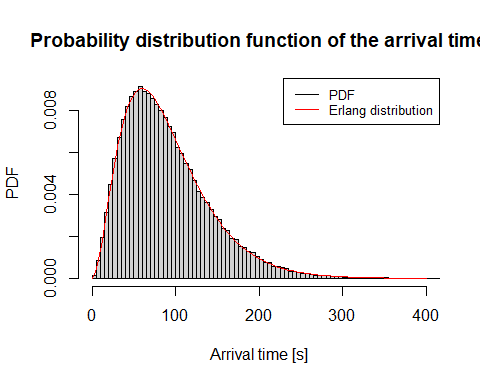
\includegraphics{Diorio_exe2_files/figure-latex/unnamed-chunk-13-1.pdf}

\begin{Shaded}
\begin{Highlighting}[]
\DocumentationTok{\#\# Repeating the same steps as point b) but evaluating the difference of time between fifth and first passenger}

\NormalTok{arrivals}\FloatTok{.2} \OtherTok{\textless{}{-}} \ControlFlowTok{function}\NormalTok{() \{}
\NormalTok{  dt1 }\OtherTok{\textless{}{-}} \FunctionTok{rexp}\NormalTok{(}\DecValTok{1}\NormalTok{, lambda)}
\NormalTok{  dt2 }\OtherTok{\textless{}{-}} \FunctionTok{rexp}\NormalTok{(}\DecValTok{1}\NormalTok{, lambda)}
\NormalTok{  dt3 }\OtherTok{\textless{}{-}} \FunctionTok{rexp}\NormalTok{(}\DecValTok{1}\NormalTok{, lambda)}
\NormalTok{  dt4 }\OtherTok{\textless{}{-}} \FunctionTok{rexp}\NormalTok{(}\DecValTok{1}\NormalTok{, lambda)}
\NormalTok{  dt5 }\OtherTok{\textless{}{-}} \FunctionTok{rexp}\NormalTok{(}\DecValTok{1}\NormalTok{, lambda)}
  
\NormalTok{  T1 }\OtherTok{\textless{}{-}}\NormalTok{ dt1 }
\NormalTok{  T5 }\OtherTok{\textless{}{-}}\NormalTok{ dt1 }\SpecialCharTok{+}\NormalTok{ dt2 }\SpecialCharTok{+}\NormalTok{ dt3 }\SpecialCharTok{+}\NormalTok{ dt4 }\SpecialCharTok{+}\NormalTok{ dt5}
  
\NormalTok{  DT }\OtherTok{\textless{}{-}}\NormalTok{ T5 }\SpecialCharTok{{-}}\NormalTok{ T1}
  
  \FunctionTok{return}\NormalTok{(DT)}
\NormalTok{\}}

\NormalTok{N\_samples}\FloatTok{.2} \OtherTok{\textless{}{-}} \DecValTok{100000}
\NormalTok{time}\FloatTok{.2} \OtherTok{\textless{}{-}} \FunctionTok{c}\NormalTok{(}\FunctionTok{rep}\NormalTok{(}\DecValTok{0}\NormalTok{, N\_samples}\FloatTok{.2}\NormalTok{))}
\ControlFlowTok{for}\NormalTok{ (i }\ControlFlowTok{in} \DecValTok{1}\SpecialCharTok{:}\NormalTok{N\_samples}\FloatTok{.2}\NormalTok{) \{}
\NormalTok{  time}\FloatTok{.2}\NormalTok{[i] }\OtherTok{\textless{}{-}} \FunctionTok{arrivals.2}\NormalTok{()}
\NormalTok{\}}

\NormalTok{x }\OtherTok{\textless{}{-}} \DecValTok{0}\SpecialCharTok{:}\NormalTok{N\_samples}\FloatTok{.2}
\FunctionTok{hist}\NormalTok{(time}\FloatTok{.2}\NormalTok{, }\AttributeTok{breaks =} \StringTok{\textquotesingle{}FD\textquotesingle{}}\NormalTok{,}
     \AttributeTok{probability =} \ConstantTok{TRUE}\NormalTok{, }\AttributeTok{xlab =} \FunctionTok{expression}\NormalTok{(Delta }\SpecialCharTok{*} \StringTok{\textquotesingle{}T \textbackslash{} [s]\textquotesingle{}}\NormalTok{), }\AttributeTok{ylab =} \StringTok{\textquotesingle{}PDF\textquotesingle{}}\NormalTok{, }
     \AttributeTok{main =} \FunctionTok{expression}\NormalTok{(}\StringTok{\textquotesingle{}Probability distribution function of \textbackslash{} \textquotesingle{}} \SpecialCharTok{*}\NormalTok{ Delta }\SpecialCharTok{*} \StringTok{\textquotesingle{}T\textquotesingle{}}\NormalTok{))}
\FunctionTok{curve}\NormalTok{(}\FunctionTok{dgamma}\NormalTok{(x, }\AttributeTok{shape =} \DecValTok{4}\NormalTok{, }\AttributeTok{rate =}\NormalTok{ lambda), }\AttributeTok{col =} \StringTok{\textquotesingle{}red\textquotesingle{}}\NormalTok{, }\AttributeTok{add =} \ConstantTok{TRUE}\NormalTok{, }\AttributeTok{xlim =} \FunctionTok{c}\NormalTok{(}\DecValTok{0}\NormalTok{, }\DecValTok{400}\NormalTok{))}
\FunctionTok{legend}\NormalTok{(}\StringTok{\textquotesingle{}topright\textquotesingle{}}\NormalTok{, }\AttributeTok{legend =} \FunctionTok{c}\NormalTok{(}\StringTok{\textquotesingle{}PDF\textquotesingle{}}\NormalTok{, }\StringTok{\textquotesingle{}Erlang distribution\textquotesingle{}}\NormalTok{),}
       \AttributeTok{col =} \FunctionTok{c}\NormalTok{(}\StringTok{\textquotesingle{}black\textquotesingle{}}\NormalTok{, }\StringTok{\textquotesingle{}red\textquotesingle{}}\NormalTok{), }\AttributeTok{lty =} \DecValTok{1}\NormalTok{, }\AttributeTok{cex =} \FloatTok{0.8}\NormalTok{)}
\end{Highlighting}
\end{Shaded}

\includegraphics{Diorio_exe2_files/figure-latex/unnamed-chunk-14-1.pdf}

\end{document}
